\let\negmedspace\undefined
\let\negthickspace\undefined
\documentclass[journal]{IEEEtran}
\usepackage[a5paper, margin=10mm, onecolumn]{geometry}
%\usepackage{lmodern} % Ensure lmodern is loaded for pdflatex
\usepackage{tfrupee} % Include tfrupee package

\setlength{\headheight}{1cm} % Set the height of the header box
\setlength{\headsep}{0mm}     % Set the distance between the header box and the top of the text

\usepackage{gvv-book}
\usepackage{gvv}
\usepackage{cite}
\usepackage{amsmath,amssymb,amsfonts,amsthm,mathtools}
\usepackage{algorithmic}
\usepackage{graphicx}
\usepackage{textcomp}
\usepackage{xcolor}
\usepackage{txfonts}
\usepackage{listings}
\usepackage{enumitem}
\usepackage{mathtools}
\usepackage{gensymb}
\usepackage{comment}
\usepackage[breaklinks=true]{hyperref}
\usepackage{tkz-euclide} 
\usepackage{listings}
\def\inputGnumericTable{}                                 
\usepackage[latin1]{inputenc}                                
\usepackage{color}                                            
\usepackage{array}                                            
\usepackage{longtable}                                       
\usepackage{calc}                                             
\usepackage{multirow}                                         
\usepackage{hhline}                                           
\usepackage{ifthen}                                           
\usepackage{lscape}
\begin{document}

\bibliographystyle{IEEEtran}
\vspace{3cm}

\title{3.2.24}
\author{EE24BTECH11020 - Ellanti Rohith
}
% \maketitle
% \newpage
% \bigskip
{\let\newpage\relax\maketitle}

\renewcommand{\thefigure}{\theenumi}
\renewcommand{\thetable}{\theenumi}
\setlength{\intextsep}{10pt} % Space between text and floats

\textbf{Question:}  A triangle $ABC$ can be constructed in which $BC = 6cm, \angle B =30\degree$ and $AC - AB=4cm$.\\

\textbf{Solution:}
\begin{table}[h!]    
  \centering
  \begin{tabular}[12pt]{ |c| c|}
    \hline
    \textbf{Variable} & \textbf{Description}\\ 
    \hline
	$\vec{e}$ & Eccentricity of conic\\
	\hline
	$\vec{F}$ & Focus of conic\\
	\hline
	$\vec{I}$ & Identity matrix\\
	\hline
	$\vec{n}^{\top}\vec{x}=c$ & Equation of directrix\\
	\hline
	$\vec{n}$ & Slope of normal to directrix\\
	\hline
	$f$ & $\norm{\vec{n}}^2\norm{\vec{F}}^2-c^2e^2$\\
	\hline
	$\vec{V}$ & A symmetric matrix given by eigenvalue decomposition\\
	\hline
	$\vec{u}$ & Vertex of conic with same directrix\\
	\hline
\end{tabular}

  \caption{Variables Used}
  
\end{table}\\
Using the cosine formula in  $\triangle ABC$,
\begin{align}
    (K + c)^2 &= a^2 + c^2 - 2ac \cos B \\
    \implies c &= \frac{a^2 - K^2}{2(K + a \cos B)}
\end{align}

Substituting the values of  K = 4 ,  a = 6 , and $\cos B = \cos 30^\circ = \frac{\sqrt{3}}{2}$ :

\begin{align}
    c &= \frac{6^2 - 4^2}{2(4 + 6 \cos 30^\circ)} \\
    c &= \frac{36 - 16}{2\left(4 + \brak{6 \times \frac{\sqrt{3}}{2}\right)}} \\
    c &= \frac{10}{4 + 3\sqrt{3}}
\end{align}

The coordinates of \( \triangle ABC \) can then be expressed as:

\begin{align}
    \vec{A} = c \myvec{\cos{B} \\ \sin{B}}, 
    \vec{B} = \myvec{0 \\ 0}, 
    \vec{C} = \myvec{a \\ 0}   
\end{align}
\begin{align}
    \vec{A} =  \frac{10}{4 + 3\sqrt{3}}\myvec{\frac{\sqrt{3}}{2} \\ \frac{1}{\sqrt{2}}}, 
    \vec{B} = \myvec{0 \\ 0}, 
    \vec{C} = \myvec{6 \\ 0}   
\end{align}

\begin{figure}[h!]
   \centering
   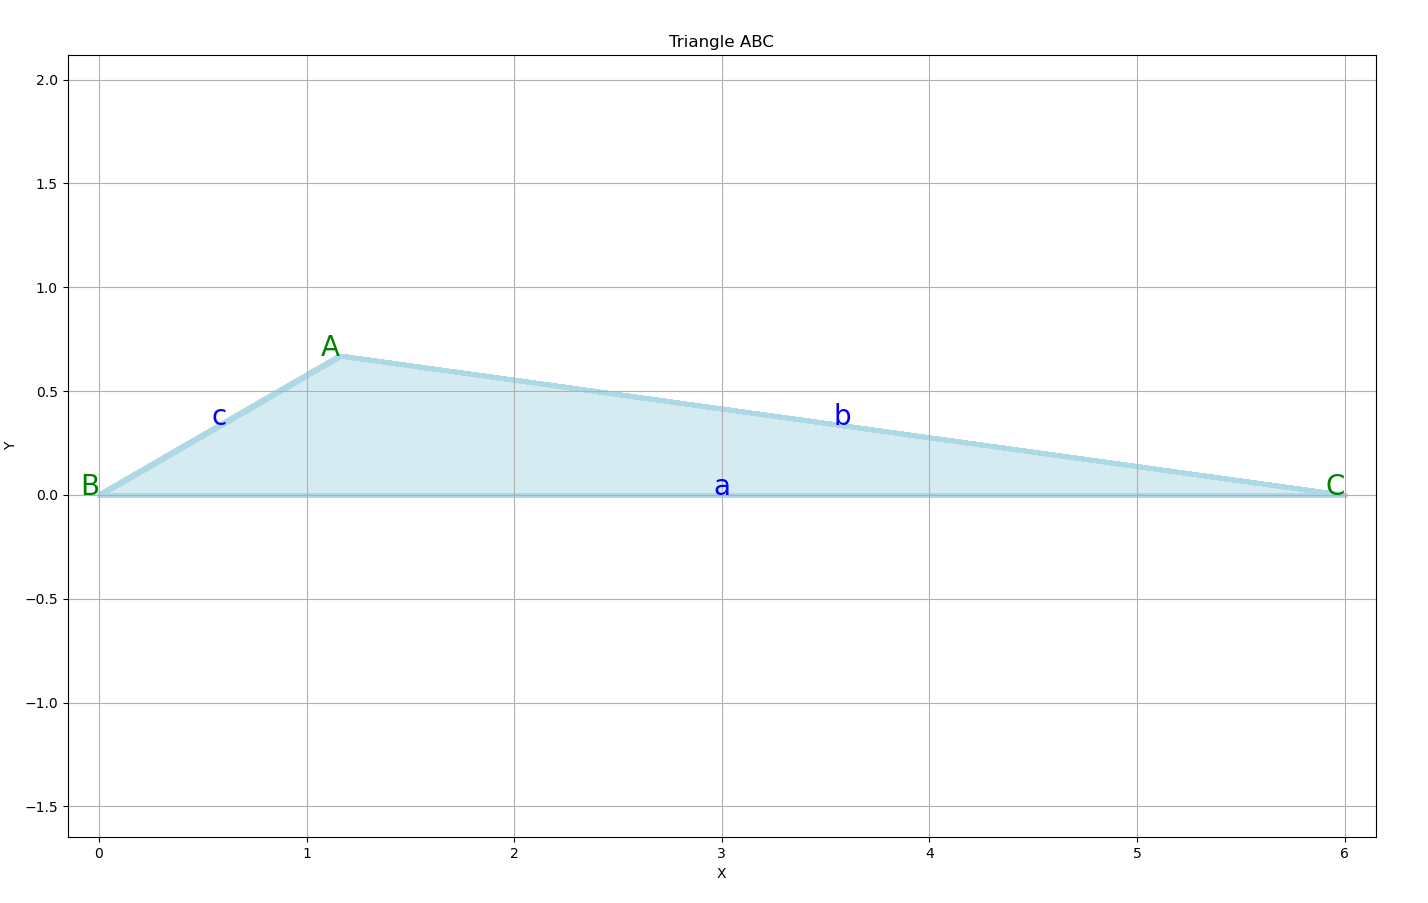
\includegraphics[width=0.7\linewidth]{figs/fig.png}
   \caption{Triangle with $BC = 6cm, \angle B =30\degree$ and $AC - AB=4cm$}
\end{figure}

\end{document}
